\section{Interpretation}
\label{sec:vergleich}
Das Paper hat das IS Success-Modell abgewandelt um MOOC Erfolg zu bemessen.  
Die Ergebnisse verdeutlichen, dass die Servicequalität einen Einfluss auf die Nutzerzufriedenheit und die Nutzerzufriedenheit wiederum einen starken Einfluss auf den Net Benefit haben (H2 und H4 bestätigt). Besser gesagt, die Betreuung durch Lehrende und Mentoren haben einen maßgeblichen Einfluss auf die Zufriedenheit der Teilnehmer eines MOOCs. Allerdings konnte keine bedeutungsvolle Beziehung zwischen der Servicequalität und dem Net Benefit ermittelt werden (H3 nicht bestätigt). Das bedeutet, dass eine gute Servicequalität nicht direkt zu einer Verbesserung des (wahrgenommenen) Erfolgs der Teilnehmer führt, sondern lediglich über einen indirekten Einfluss verfügt (Servicequalität $\rightarrow$ Nutzerzufriedenheit $\rightarrow$ Net Benefit; $\gamma$ = 0,333). Überraschend ist auch, dass die Systemqualität keine ausschlaggebende Wirkung auf die Nutzerzufriedenheit aufweist, obwohl diese in vergangenen Studien durchaus Einfluss nachgewiesen werden konnte \parencite{freeze2010success, islam2013investigating, mohammadi2015factors}. 
Auffällig ist auch, dass die R$^2$-Werte lediglich im "`mittelguten"' Bereich liegen \parencite[vgl.][S.323]{chin1998partial}. Dies ist ein Zeichen, dass es womöglich noch andere Faktoren gibt, die die Variablen Nutzerzufriedenheit und Net Benefit beschreiben könnten \parencite[vgl.][S.179]{freeze2010success}.  
Zusammenfassend gesagt, die IS Success-Perspektive scheint nur ein Teil des MOOC Erfolgs zu erklären. Zum besseren Verständnis bedarf es einer Erweiterung des Modells. In vergangenen Studien wurde bereits das Technology-Acceptance-Modell (TAM) von \textcite{bagozzi1992development} als eine sinnvolle Ergänzung zum IS Success Modell im e-Learning-Bereich identifiziert \parencite{mohammadi2015factors} und könnte auch auf MOOCs anwendbar sein. Es wird vorwiegend angewandt um Faktoren zu analysieren, die Nutzer zur Nutzung einer neuen Technologie bewegen \parencite[vgl.][S.702]{mohammadi2015factors}.  
Aus einer etwas anderen Richtung käme das Community of Inquiry(COI)-Modell von \textcite{garrison1999critical}. Es besteht aus den drei Komponenten "`cognitive"',  "`social"' und "`teaching presence"' die in der "`educational experience"'  münden. Die "`Educational Experience"' kann dabei aus der IS Success Perspektive als Nutzerzufriedenheit oder Net Benefit interpretiert werden und damit die Verbindung der beiden Modelle herstellen.  

The COI model urges a more integrative role of both the student and teacher through a balance in each of the three presences of computer mediated communication. An increased understanding of the educational experience may occur through an understanding of how students construct meaning through sustained communication (Cognitive presence), project personal characteristics (Social presence), and realize personal meaning (Teaching presence). The COI model may help educators to understand the environment created by the ELS that facilitates the online learning experience.

Da ein MOOC zumeist ein von Universitäten angebotener Kurs, der bei erfolgreichem Abschluss Credit-points gutschreibt und ein Zertifikat ausstellt, liegt es nahe, den Bildungscharakter des MOOC mithilfe des COI-Modells zu analysieren.     

Limitationen und Ausblick
Als eine der ersten im Rahmen von MOOCs durchgeführten Studien weist das Paper einige Limitation auf. Die untersuchte Stichprobe ist begrenzt auf einen MOOC einer Universität. Es ist eine größere Stichprobe und eine Erweiterung der Studie auf andere Universitäten, bzw. andere MOOCs nötig, um eine Verallgemeinerung der Ergebnisse zu legitimieren. Des Weiteren bezieht sich die Studie auf eine bestimmte Form eines MOOCs: einen Mentored Open Online Course. Der besondere Fokus auf die Servicequalität sollte im Vergleich zum üblichen Massive Open Online Course Beachtung entgegengebracht werden. Die große Varietät der MOOC-Teilnehmer in Alter und Herkunft kann ebenfalls zu Verzerrungen der Ergebnisse führen, da unterschiedliche Kulturen, Berufserfahrung, oder Bildung zu unterschiedlichen Ansprüchen führen. 
Ferner kann eine Integration andere Aspekte wie z.B. menschliche Faktoren (Charaktereigenschaften), Thematik des Kurses oder die Arbeitsweise (Teamarbeit, Einzelarbeit) neue Perspektiven eröffnen, die die Aussagekraft des Modell erhöhen. Besonders die Vielfalt in Alter und Herkunft bei MOOCs bietet eine gute Basis um beispielsweise kulturelle Aspekte zu analysieren.  

schlusssatz

 

The story of MOOCs is not going to be told with conventional statistics borrowed from brick-and-mortar classroom models. Rather, our research describes an emerging learning ecosystem, one where enrollment can be casual and nonbinding, learning happens asynchronously, and registrants come from all countries in the world, with diverse intentions and patterns of learning. The metrics we choose should respect their intentions and encourage their learning.\parencite{reich2014tricky}


\begin{figure}[h]
\centering
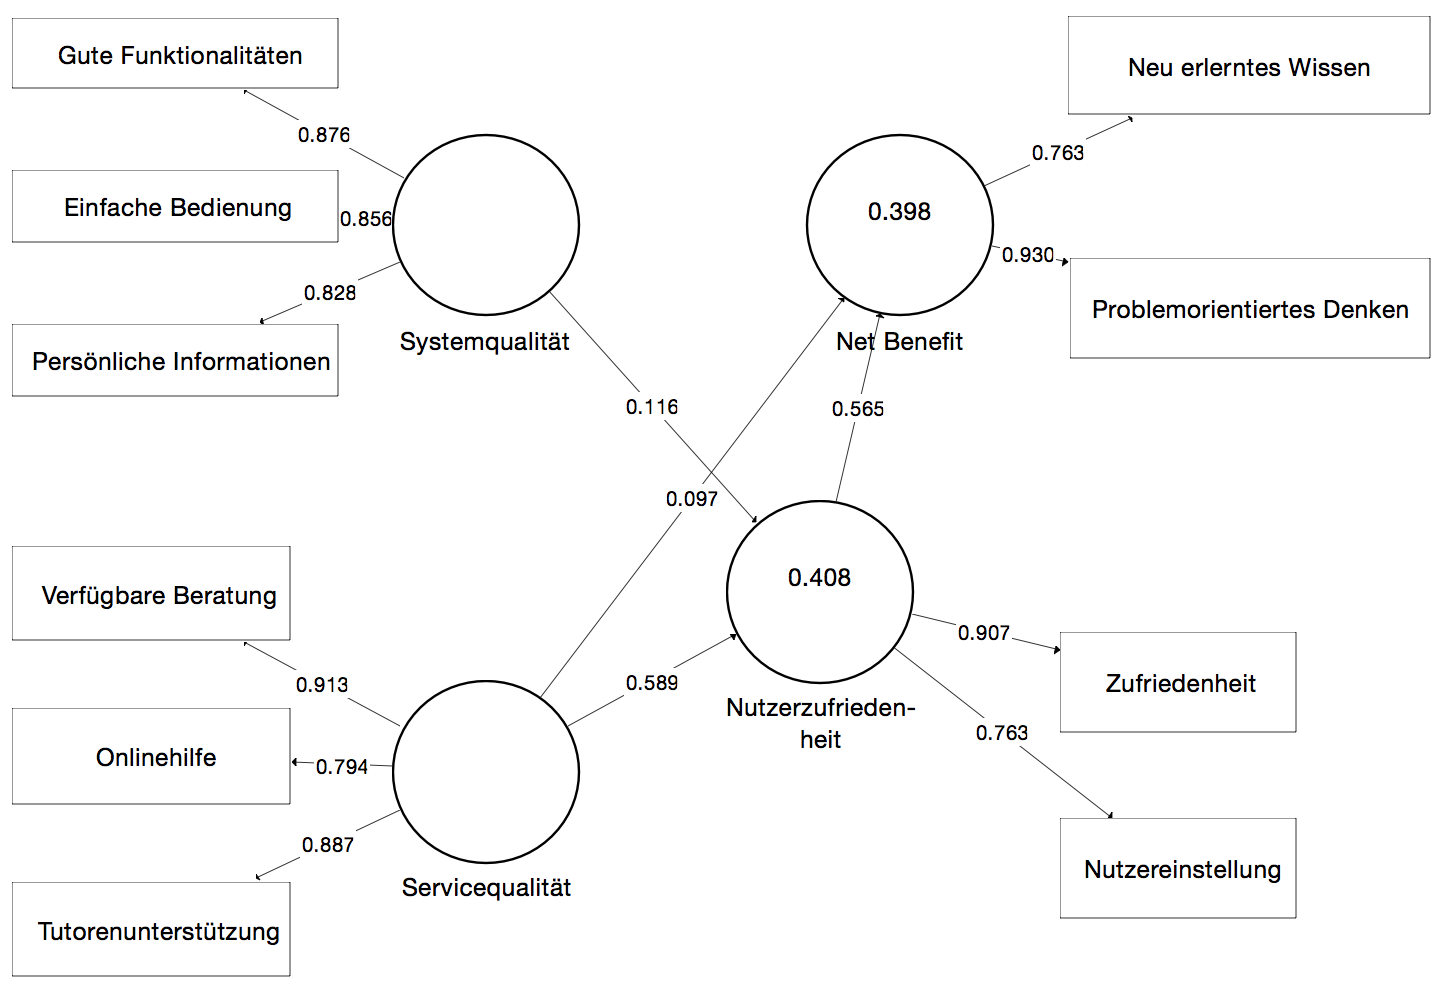
\includegraphics[width=1\textwidth]{Grafiken/pls_bw_3.png}
\caption{PLS Modellergebnisse}
\label{PLS Modellergebnisse}
\end{figure}